\documentclass{beamer}
\usepackage{tipa}
\usepackage{phonrule}
%\setbeamersize{text margin left=10pt,text margin right=10pt}
\usetheme{metropolis}
\usepackage{listings}
\usepackage{amsfonts}
\usepackage{dsfont}
\usepackage{amsmath}
\usepackage{bbm}
\usepackage{verbatim}
\usepackage{phonrule}
%\usepackage{tipa}
\usepackage{tikz}
\usetikzlibrary{fit}
\usepackage{color}
\usepackage{booktabs}
\usepackage{tipa}
\usepackage{amssymb}
\usepackage{verbatim}
\usepackage[absolute,overlay]{textpos}
\usepackage{pifont}% http://ctan.org/pkg/pifont
\usepackage{caption}
\usepackage{subcaption}
\newcommand{\cmark}{\ding{51}}%
\newcommand{\xmark}{\ding{55}}%
\usetikzlibrary{bayesnet}
\usetikzlibrary{decorations.markings}
\usetikzlibrary{decorations.pathmorphing}
\tikzset{squiggle/.style={decorate, decoration={snake,amplitude=.4mm}}}
\usepackage{xcolor}
\definecolor{pop1}{HTML}{1F78b4}
\definecolor{pop2}{HTML}{164C13}
\definecolor{pop3}{HTML}{d95F02}
\definecolor{orange}{HTML}{d95F02}
\definecolor{teal}{HTML}{1b9e77}
\newcommand{\pop}[1]{\textcolor{pop1}{#1}}
\newcommand{\popp}[1]{\textcolor{pop2}{#1}}
\newcommand{\tree}[1]{\textcolor{pop3}{#1}}
\newcommand{\orange}[1]{\textcolor{orange}{#1}}
\newcommand{\teal}[1]{\textcolor{teal}{#1}}
\newcommand{\code}[1]{{\footnotesize\texttt{#1}}}
\newcommand{\greenCode}[1]{{\footnotesize\popp{\code{#1}}}}
\newcommand{\blueCode}[1]{{\footnotesize\pop{\code{#1}}}}
\definecolor{backgroundGreen}{HTML}{23373b}
\lstset{escapeinside={<@}{@>}}
\usepackage{pgf}  

%% \usepackage[sfdefault]{FiraSans} %% option 'sfdefault' activates Fira Sans as the default text font
%% \usepackage[T1]{fontenc}
%% \renewcommand*\oldstylenums[1]{{\firaoldstyle #1}}


\newcommand{\Expect}{\mathds{E}} %{{\rm I\kern-.3em E}}
\newcommand{\1}[1]{\mathds{1}\left[#1\right]}
\newcommand{\E}{\mathds{E}} %{{\rm I\kern-.3em E}}
\newcommand{\indicator}{\mathds{1}} %{{\rm I\kern-.3em E}}
\newcommand{\expect}{\mathds{E}} %{{\rm I\kern-.3em E}}
\newcommand{\probability}{\mathds{P}} %{{\rm I\kern-.3em P}}
\DeclareMathOperator*{\argmin}{arg\,min} % thin space, limits underneath in displays
\DeclareMathOperator*{\argmax}{arg\,max} % thin space, limits underneath in displays
\DeclareMathOperator*{\argmaxk}{arg\,top-\textit{k}} % thin space, limits underneath in displays

\usepackage[absolute,overlay]{textpos}

\newcommand{\nextForm}[1]{\rotatebox[origin=c]{270}{$_{\curvearrowright}$}$_{#1}$}
 
\usepackage{amsfonts}
\usepackage{tabularx}
%\usepackage{color}
\usepackage{graphicx}
\usepackage{booktabs}
\usepackage{xcolor}
\usepackage{tikz}
\usetikzlibrary{trees}
\usetikzlibrary{fit}
\usetikzlibrary{calc}
\usetikzlibrary{bayesnet}
\usepackage[absolute,overlay]{textpos}
\usepackage{stmaryrd}
\newcommand{\sem}[1]{\llbracket #1\rrbracket}
\newcommand{\eval}[1]{\llbracket #1\rrbracket}
\newcommand{\tuple}[1]{\ensuremath{\left \langle #1\right \rangle}}
\newcommand{\messageOverlay}[1]{
      \tikz[overlay,remember picture]
      \node[align=left,fill=backgroundGreen,text=white] at (current page.center){#1};
}
\newcommand{\myPaper}[1]{
  \tikz[overlay,remember picture]
  \node[anchor=south west,align=left] at (current page.south west){#1};
}
\newcommand{\myPaperRight}[1]{
  \tikz[overlay,remember picture]
  \node[anchor=south east,align=left] at (current page.south east){#1};
}
\usepackage{booktabs}
\usepackage{tipa}
\usepackage{amssymb}
\usepackage{verbatim}
\usepackage[absolute,overlay]{textpos}
\usepackage{pifont}% http://ctan.org/pkg/pifont
%% \newcommand{\cmark}{\ding{51}}%
%% \newcommand{\xmark}{\ding{55}}%
\usetikzlibrary{bayesnet}
\usetikzlibrary{decorations.markings}

\newcommand\Wider[2][3em]{%
\makebox[\linewidth][c]{%
  \begin{minipage}{\dimexpr\textwidth+#1\relax}
  \raggedright#2
  \end{minipage}%
  }%
}
\definecolor{backgroundBeige}{RGB}{250,250,250}
\newcommand{\denotation}[1]{{\llbracket #1 \rrbracket}}

\usepackage[utf8]{inputenc}
\newcommand{\reduce}{\longrightarrow}
\usepackage{amssymb}% http://ctan.org/pkg/amssymb
\usepackage{pifont}% http://ctan.org/pkg/pifont

\usepackage{fancyvrb}

\usepackage[most]{tcolorbox}
\definecolor{block-gray}{gray}{0.10}
\newtcolorbox{mycode}{colback=block-gray,grow to right by=0mm,grow to left
by=0mm, boxrule=0pt,boxsep=0pt,breakable,fontupper=\color{white}}

%% Program ::=
%%   (if Bool List
%%     (append RecursiveList
%%             RecursiveList
%%             RecursiveList))
%% RecursiveList ::= List
%%          | (recurse List)

            

\usepackage{arydshln}

%\newcommand{\Expect}{\mathds{E}} %{{\rm I\kern-.3em E}}
\newcommand{\Probability}{\mathds{P}} %{{\rm I\kern-.3em P}}

%\DeclareMathOperator*{\argmax}{arg\,max}
%Information to be included in the title page:
\title{DreamCoder: Growing domain-specific knowledge via wake-sleep program induction} %DreamCoder:\\Growing generalizable, interpretable knowledge with wake-sleep Bayesian program learning}
\author{Kevin Ellis\\Collaborators: Catherine Wong, Maxwell Nye, Mathias Sabl\'e-Meyer,\\  Lucas Morales, Armando Solar-Lezama, Joshua B. Tenenbaum}
\institute{Conceptual Abstraction and Analogy in Natural and Artificial Intelligence}
\date{2020}
  
 
\begin{document}
 
\frame{\titlepage}

\begin{frame}{The premise of program induction}

  1. Represent knowledge as programs: as symbolic code

  \pause

  \vspace{1cm}

  2. Learning$ = $adding to that body of knowledge$ = $ \phantom{testtesttest}%
  making new programs$ = $program synthesis

\end{frame}

\begin{frame}{Why program induction?}
  \Wider[6.5em]{  \begin{tabular}{ccc}
    \visible<2->{\begin{tabular}{l}
      strong generalization\\
      +data efficiency
    \end{tabular}}&
    \visible<3->{\begin{tabular}{l}
        compositional reuse\\
        of abstractions
    \end{tabular}}
    &\visible<4->{\begin{tabular}{l}
       universal expressivity\\
     \end{tabular}}\\
    \visible<2->{
      \begin{tabular}{c}
        \includegraphics[width = 3cm]{figures/polynomialExtrapolation}\\
        {\small\texttt{f(x)=(x-1)**2 - 0.5}}
    \end{tabular}}&
    \visible<3->{\begin{tabular}{c}
        \includegraphics[width = 3.5cm]{figures/explodedCAD}\\\emph{vs}\\
        \includegraphics[width = 3.5cm]{figures/drillMesh}
    \end{tabular}}&
    \visible<4->{%% \includegraphics[width = 4cm]{figures/turingMachine}
      \begin{tabular}{c}
        \includegraphics[width = 3cm]{figures/famous}
    \end{tabular}}
  \end{tabular}}
\end{frame}


\begin{frame}{}
  \Wider[5em]{  \begin{tabular}{cc}
      FlashFill (Gulwani 2012)&\\
      \begin{tabular}{c}
        \includegraphics[width = 6cm]{ff_example}
      \end{tabular}&
      \begin{tabular}{c}
        \visible<3->{\includegraphics[width = 5cm]{ff_DSL}}
      \end{tabular}\\
      \visible<2->{Szalinski (Nandi 2020)}&\\
      \begin{tabular}{c}
        \visible<2->{\includegraphics[width = 6cm]{uwCAD_example}}
      \end{tabular}&
      \begin{tabular}{c}
        \visible<3->{\includegraphics[width = 5cm]{uwCAD_DSL}}
      \end{tabular}
  \end{tabular}}
\end{frame}

\begin{frame}{Program induction for learning and perception}
  \begin{tikzpicture}
    \node at(0,0) {\includegraphics[width = 8cm]{../ecPaper/characters.png}};
    \node at(-3,2) {\includegraphics[width = 8cm]{../ecPaper/Brendan.jpg}};

    \node at (-5,-4) {  Lake et al 2015};
    \end{tikzpicture}
\end{frame}




\begin{frame}{}
  \begin{center}
    \begin{tabular}{l}
      {\textcolor{black}{Program Induction and {\textcolor{black}{learning to learn}}}}\\
      {\phantom{Program Induction and }\textcolor{gray}{learning a DSL}}\\
      {\phantom{Program Induction and }\textcolor{gray}{learning to synthesize}}\\
      {\phantom{Program Induction and }{\textcolor{gray}{synergy between DSL+learned synthesizer}}}\\
    \end{tabular}
  \end{center}
\end{frame}



\begin{frame}{Learning to write code} %Growing domain-specific knowledge}
  
  %  \Large
  Goal: acquire domain-specific knowledge needed to induce a class of programs


  
  \vspace{0.75cm}

  \Wider[4em]{
    \begin{itemize}
    \item Library of abstractions (domain specific language) \\ %; generative model over programs)
      \item      Inference strategy (synthesis algorithm)
      \end{itemize}
  }
  
  \vspace{0.75cm}
  
  \visible<2>{
  \begin{tikzpicture}
    \node(problem) at (0,0) {\includegraphics[width = 2cm]{figures/cubic.png}};
    \node(synthesizer)[draw,align=center] at ([xshift=3cm]problem.east) {Learned \\program inducer};
    \draw[->] (problem.east) -- (synthesizer.west);
    \node(program)[draw, align=center] at ([xshift=3cm]synthesizer.east) {program:\\$f(x) = 0.3x^3+$\\$1.1x^2-2x+0.6$};
    \draw[->] (synthesizer.east) -- (program.west);
  \end{tikzpicture}
  
    \vspace{0.2cm}Concepts: $x^3$, $\alpha x + \beta$, etc\\Inference strategy: neurosymbolic search for programs}
  %% \renewcommand\code\texttt
  %%   \only<3>{
  %% \begin{tikzpicture}
  %%   \node(problem) at (0,0) {\includegraphics[width = 2cm]{figures/radialCircle.png}};
  %%   \node(synthesizer)[draw,align=center] at ([xshift=3cm]problem.east) {Learned \\program inducer};
  %%   \draw[->] (problem.east) -- (synthesizer.west);
  %%   \node(program)[draw, align=center] at ([xshift=3cm]synthesizer.east) {program:\\\code{(radial-symmetry 5}\\\code{ (circle 3))}};
  %%   \draw[->] (synthesizer.east) -- (program.west);
  %% \end{tikzpicture}
  
  %% \vspace{0.2cm}Concepts: \code{circle}, \code{radial-symmetry}, etc\\Inference strategy: neurosymbolic search for programs
  %%   }
\end{frame}


\begin{frame}{Library learning}
  \Wider[5em]{
    \begin{center}
      \begin{tabular}{cc}
        \includegraphics[height=\textheight]{figures/figureOneFinal1_primitives}&
        \includegraphics[height=\textheight]{figures/figureOneFinal1_problem}
      \end{tabular}
    \end{center}
  }
  \myPaper{Ellis, Morales, Sable-Meyer, Solar-Lezama, Tenenbaum. NeurIPS 2018.\\
    Ellis, Wong, Nye, ..., Solar-Lezama, Tenenbaum. arxiv 2020.}
\end{frame}

\begin{frame}[t]{Library learning}
\Wider[5em]{  \begin{center}
    \begin{tabular}{ccc}
      \includegraphics[height=0.6\textheight]{figures/figureOneFinal1_primitives}&
      \phantom{testingtesting}&
      \includegraphics[height=0.6\textheight]{figures/figureOneFinal1_problem}
    \end{tabular}
\end{center}}
\myPaper{Ellis, Wong, Nye, ..., Solar-Lezama, Tenenbaum. arxiv 2020.}
\end{frame}


\begin{frame}{Library learning}
%  \centering
  
  \only<1>{  \Wider[5em]{\includegraphics[width = \textwidth]{figures/figureOneFinal1}}}
  \only<2>{  \Wider[5em]{\includegraphics[width = \textwidth]{figures/figureOneFinal2_layer1}}}
  \only<3>{  \Wider[5em]{\includegraphics[width = \textwidth]{figures/figureOneFinal2_layer1_exploded}}}
  \only<4>{  \Wider[5em]{\includegraphics[width = \textwidth]{figures/figureOneFinal2_layer1}}}
  \only<5>{  \Wider[5em]{\includegraphics[width = \textwidth]{figures/figureOneFinal2_layer2}}}
  \only<6>{  \Wider[5em]{\includegraphics[width = \textwidth]{figures/figureOneFinal2_layer2_exploded}}}
  \only<7>{  \Wider[5em]{\includegraphics[width = \textwidth]{figures/figureOneFinal2_layer2}}}
  \only<8>{  \Wider[5em]{\includegraphics[width = \textwidth]{figures/figureOneFinal2}}}
  \only<9>{  \Wider[5em]{\includegraphics[width = \textwidth]{figures/figureOneFinal2_exploded}}}
  \only<10>{  \Wider[5em]{\includegraphics[width = \textwidth]{figures/figureOneFinal3}}}
  \only<11>{  \Wider[5em]{\includegraphics[width = \textwidth]{figures/figureOneFinal3_explained_exploded}}}
  \only<12->{  \Wider[5em]{\includegraphics[width = \textwidth]{figures/figureOneFinal3_explained}}}
%  \only<12>{  \Wider[5em]{\includegraphics[width = \textwidth]{figures/figureOneFinal4}}}
  %  \only<5>{  \Wider[5em]{\includegraphics[width = \textwidth]{figures/figureOneFinal5}}}

  \visible<12->{Solution rewritten in initial primitives:

    \tiny\texttt{(lambda (x) (map (lambda (y) (car (fold (fold x nil (lambda (z u) (if (gt? (+ y 1) (length (fold x nil (lambda (v w) (if (gt? z v) (cons v w) w))))) (cons z u) u))) nil (lambda (a b) (if (nil? (fold (fold x nil (lambda (c d) (if (gt? (+ y 1) (length (fold x nil (lambda (e f) (if (gt? c e) (cons e f) f))))) (cons c d) d))) nil (lambda (g h) (if (gt? g a) (cons g h) h)))) (cons a b) b))))) (range (length x))))}}

  \visible<13>{\normalsize induced sort program found in $\leq 10$min. Brute-force search without learned library would take $\approx 10^{73}$ years }

  \myPaper{Ellis, Wong, Nye, ..., Solar-Lezama, Tenenbaum. arxiv 2020.}
  
\end{frame}

\begin{frame}{DreamCoder}
  \begin{itemize}
  \item   \textbf{Wake:} Solve problems by writing programs
  \item \textbf{Sleep:} Improve library and neural recognition model:
    \begin{itemize}
    \item \textbf{Abstraction sleep:} Improve library
      \item \textbf{Dream sleep:} Improve neural recognition model
    \end{itemize}
%  \item   Combines ideas from Wake-Sleep \& Exploration-Compression % \& Program analysis
  \end{itemize}
  \Wider[5.4em]{
    \begin{center}
      \begin{tikzpicture}
%    \visible<2->{
      %      \node(Lisp) at (-3,0) {\includegraphics[width = 0.8\textwidth]{figures/manyDomains_child.png}};
    %%   \node[align=left,anchor=left](Lisp) at (-1,1) {Memory consolidation during human sleep:\\
    %%     1. Slow-wave ($\sim$explicit, declarative)\\
    %%   2. Fast-wave REM ($\sim$implicit, procedural)};
    %% }
%    \node at (0.9,1.3) {  \includegraphics[width = 4cm]{ecFigures/sleepingChild.jpg}};
  \end{tikzpicture}
        \end{center}}

\hspace*{-0.4cm}\small cf. Helmholtz machine, wake/sleep neural network training algorithms
\end{frame}
\begin{frame}[t]{Library learning as Bayesian inference}
  %  \includegraphics[width = 11cm]{ecFigures/animation/EC.eps}
\centering  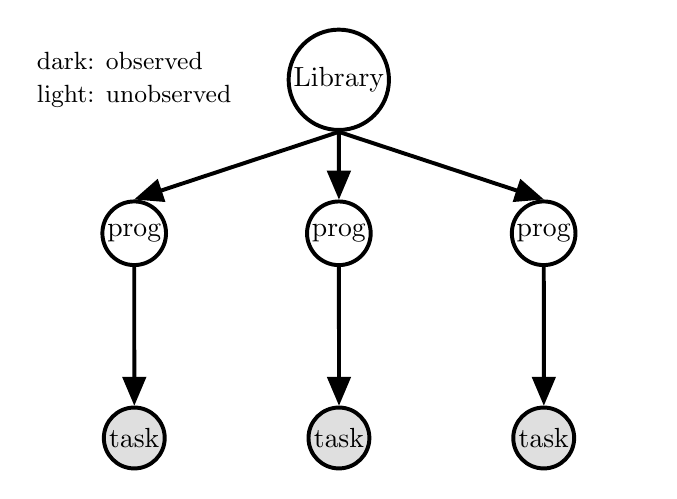
\begin{tikzpicture}[scale=1.3,line width=0.5mm]
\node[align=left] at (1.5,3) {\small dark: observed\\\small light: unobserved};
  \node[latent,scale=1] at (3.5,3) (dx){Library};
  \node[latent,scale=1] at ([yshift=-1.5cm]dx) (zp){prog};
  \node[obs,scale=1] at ([yshift=-2cm]zp) (xp) {task};
  \node[latent,scale=1] at ([xshift=2cm]zp) (zp1){prog};
  \node[obs,scale=1] at ([xshift=2cm]xp) (xp1) {task};
  \draw [->] (zp1.south) -- (xp1.north);
  \draw [->] (dx.south) -- (zp1.north);
  \draw [->,red,opacity=0.0001] (xp1.east) to[out = 30,in = -30] node(nn){} (zp1.east);
  
  \node[latent,scale=1] at ([xshift=-2cm]zp) (zp1){prog};
  \node[obs,scale=1] at ([xshift=-2cm]xp) (xp1) {task};
  \draw [->] (zp1.south) -- (xp1.north);
  \draw [->] (dx.south) -- (zp1.north);
  \draw [->] (dx.south) -- (zp.north);
  \draw [->] (zp.south) -- (xp.north);


  \end{tikzpicture}
  

\vspace{0.5cm}
  
[Dechter et al, 2013]  [Liang et al, 2010] [Lake et al, 2015]

%\textbf{Dechter et al.}: Exploration-Compression. Inspiration for DreamCoder.

  %% \vfill
  %% Gray: Observed.\\
  %% White: Latent.\\
  %% Boxed (plate): Repeated.\\
  
\end{frame}
\begin{frame}[t]{Library learning as Bayesian inference}
  %  \includegraphics[width = 11cm]{ecFigures/animation/EC.eps}
\centering  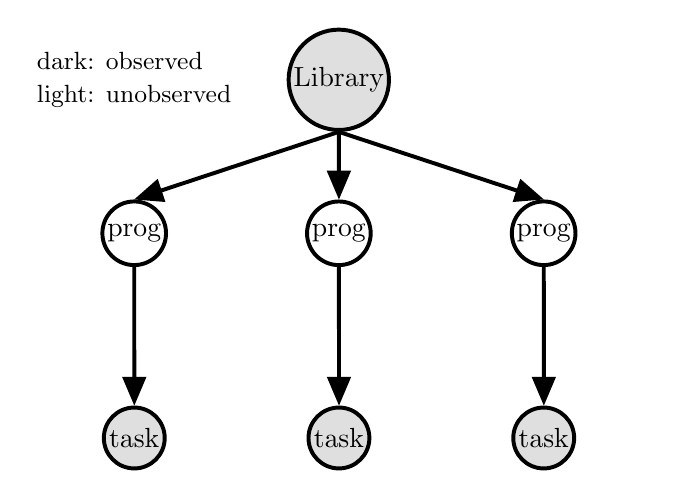
\begin{tikzpicture}[scale=1.3,line width=0.5mm]
\node[align=left] at (1.5,3) {\small dark: observed\\\small light: unobserved};
  \node[obs,scale=1] at (3.5,3) (dx){Library};
  \node[latent,scale=1] at ([yshift=-1.5cm]dx) (zp){prog};
  \node[obs,scale=1] at ([yshift=-2cm]zp) (xp) {task};
  \node[latent,scale=1] at ([xshift=2cm]zp) (zp1){prog};
  \node[obs,scale=1] at ([xshift=2cm]xp) (xp1) {task};
  \draw [->] (zp1.south) -- (xp1.north);
  \draw [->] (dx.south) -- (zp1.north);
  \draw [->,red,opacity=0.0001] (xp1.east) to[out = 30,in = -30] node(nn){} (zp1.east);
  
  \node[latent,scale=1] at ([xshift=-2cm]zp) (zp1){prog};
  \node[obs,scale=1] at ([xshift=-2cm]xp) (xp1) {task};
  \draw [->] (zp1.south) -- (xp1.north);
  \draw [->] (dx.south) -- (zp1.north);
  \draw [->] (dx.south) -- (zp.north);
  \draw [->] (zp.south) -- (xp.north);


  \end{tikzpicture}
  

\vspace{0.5cm}
  
\textbf{[Dechter et al, 2013]}  [Liang et al, 2010] [Lake et al, 2015]

%\textbf{Dechter et al.}: Exploration-Compression. Inspiration for DreamCoder.

  %% \vfill
  %% Gray: Observed.\\
  %% White: Latent.\\
  %% Boxed (plate): Repeated.\\
  
\end{frame}
\begin{frame}[t]{Library learning as Bayesian inference}
  %  \includegraphics[width = 11cm]{ecFigures/animation/EC.eps}
\centering  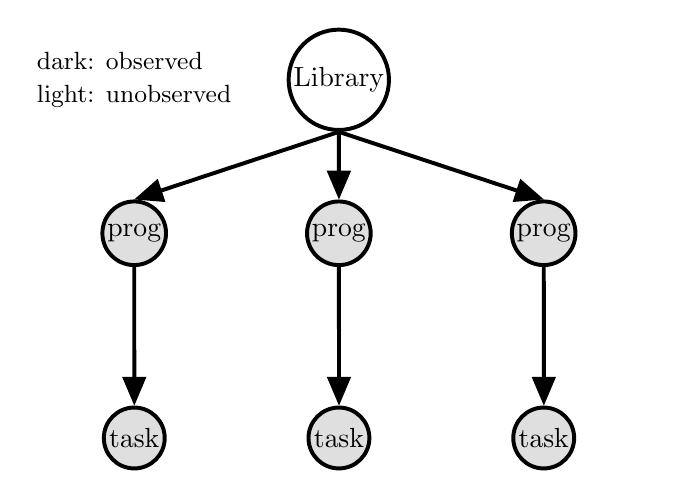
\begin{tikzpicture}[scale=1.3,line width=0.5mm]
\node[align=left] at (1.5,3) {\small dark: observed\\\small light: unobserved};
  \node[latent,scale=1] at (3.5,3) (dx){Library};
  \node[obs,scale=1] at ([yshift=-1.5cm]dx) (zp){prog};
  \node[obs,scale=1] at ([yshift=-2cm]zp) (xp) {task};
  \node[obs,scale=1] at ([xshift=2cm]zp) (zp1){prog};
  \node[obs,scale=1] at ([xshift=2cm]xp) (xp1) {task};
  \draw [->] (zp1.south) -- (xp1.north);
  \draw [->] (dx.south) -- (zp1.north);
  \draw [->,red,opacity=0.0001] (xp1.east) to[out = 30,in = -30] node(nn){} (zp1.east);
  
  \node[obs,scale=1] at ([xshift=-2cm]zp) (zp1){prog};
  \node[obs,scale=1] at ([xshift=-2cm]xp) (xp1) {task};
  \draw [->] (zp1.south) -- (xp1.north);
  \draw [->] (dx.south) -- (zp1.north);
  \draw [->] (dx.south) -- (zp.north);
  \draw [->] (zp.south) -- (xp.north);


  \end{tikzpicture}
  

\vspace{0.5cm}
  
\textbf{[Dechter et al, 2013]}  [Liang et al, 2010] [Lake et al, 2015]

%\textbf{Dechter et al.}: Exploration-Compression. Inspiration for DreamCoder.

  %% \vfill
  %% Gray: Observed.\\
  %% White: Latent.\\
  %% Boxed (plate): Repeated.\\
  
\end{frame}
\begin{frame}[t]{Library learning as Bayesian inference}
  %  \includegraphics[width = 11cm]{ecFigures/animation/EC.eps}
\centering  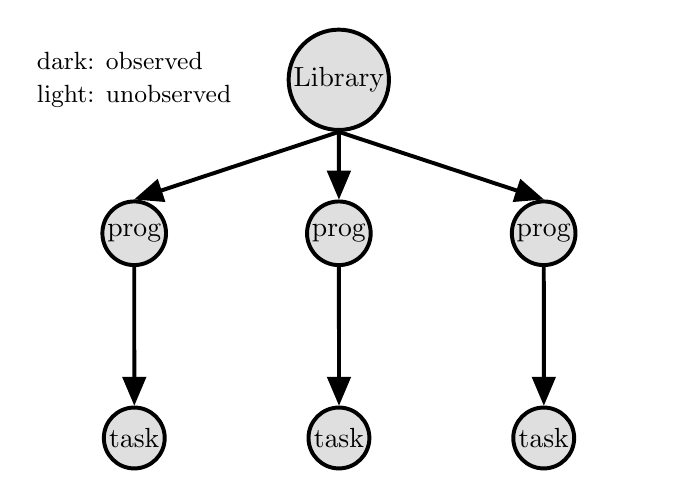
\begin{tikzpicture}[scale=1.3,line width=0.5mm]
\node[align=left] at (1.5,3) {\small dark: observed\\\small light: unobserved};
  \node[obs,scale=1] at (3.5,3) (dx){Library};
  \node[obs,scale=1] at ([yshift=-1.5cm]dx) (zp){prog};
  \node[obs,scale=1] at ([yshift=-2cm]zp) (xp) {task};
  \node[obs,scale=1] at ([xshift=2cm]zp) (zp1){prog};
  \node[obs,scale=1] at ([xshift=2cm]xp) (xp1) {task};
  \draw [->] (zp1.south) -- (xp1.north);
  \draw [->] (dx.south) -- (zp1.north);
  \draw [->,red,opacity=0.0001] (xp1.east) to[out = 30,in = -30] node(nn){} (zp1.east);
  
  \node[obs,scale=1] at ([xshift=-2cm]zp) (zp1){prog};
  \node[obs,scale=1] at ([xshift=-2cm]xp) (xp1) {task};
  \draw [->] (zp1.south) -- (xp1.north);
  \draw [->] (dx.south) -- (zp1.north);
  \draw [->] (dx.south) -- (zp.north);
  \draw [->] (zp.south) -- (xp.north);


  \end{tikzpicture}
  

\vspace{0.5cm}
  
\textbf{[Dechter et al, 2013]}  [Liang et al, 2010] [Lake et al, 2015]

%\textbf{Dechter et al.}: Exploration-Compression. Inspiration for DreamCoder.

  %% \vfill
  %% Gray: Observed.\\
  %% White: Latent.\\
  %% Boxed (plate): Repeated.\\
  
\end{frame}
\newcommand{\NeuralNetwork}[1]{    \begin{tikzpicture}[x=2.5cm,y=1.25cm,transform canvas={scale=#1,shift={+(-1,2.5)}}]
      \tikzstyle{neuron}=[circle,fill=blue!50,minimum size=20pt]
      \fill[fill=white] (-0.25,-0.5) rectangle (2.25,-4.5);
      \node[rectangle] at (1,1) {};
      \foreach \name / \y in {1,...,4}
          \node[neuron] (I-\name) at (0,-\y) {};
      \foreach \name / \y in {1,...,3}
          \node[neuron] (H-\name) at (1,-\y-0.5) {};
      \foreach \name / \y in {1,...,4}
          \node[neuron] (O-\name) at (2,-\y) {};
      \foreach \source in {1,...,4}
          \foreach \dest in {1,...,3}
              \draw [-latex] (I-\source) -- (H-\dest);
      \foreach \source in {1,...,3}
          \foreach \dest in {1,...,4}
              \draw [-latex] (H-\source) -- (O-\dest);
    \end{tikzpicture}}
\begin{frame}[t]{Library learning as \alert{neurally-guided} Bayesian inference}
\centering  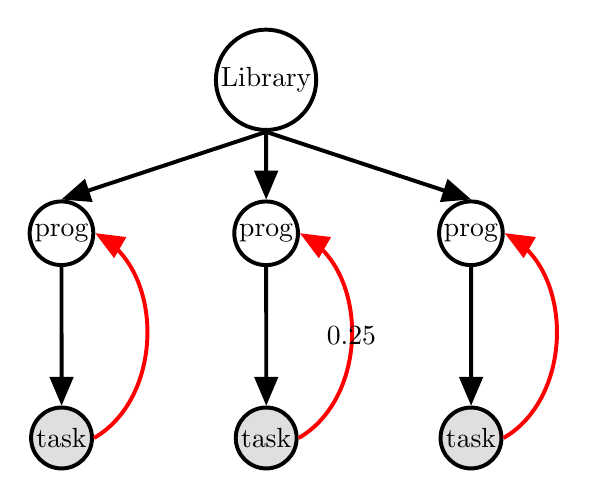
\begin{tikzpicture}[scale=1.3,line width=0.5mm]

  \node[latent,scale=1] at (3.5,3) (dx){Library};
  \node[latent,scale=1] at ([yshift=-1.5cm]dx) (zp){prog};
  \node[obs,scale=1] at ([yshift=-2cm]zp) (xp) {task};
  \node[latent,scale=1] at ([xshift=2cm]zp) (zp1){prog};
  \node[obs,scale=1] at ([xshift=2cm]xp) (xp1) {task};
  \draw [->] (zp1.south) -- (xp1.north);
  \draw [->] (dx.south) -- (zp1.north);
  \draw [->,red] (xp1.east) to[out = 30,in = -30] node(nn){} (zp1.east);
%  \node at (nn) {\NeuralNetwork{0.5}};
  
  \node[latent,scale=1] at ([xshift=-2cm]zp) (zp1){prog};
  \node[obs,scale=1] at ([xshift=-2cm]xp) (xp1) {task};
  \draw [->] (zp1.south) -- (xp1.north);
  \draw [->] (dx.south) -- (zp1.north);
  \draw [->,red] (xp1.east) to[out = 30,in = -30] node(nn){} (zp1.east);
%  \node at (nn) {\NeuralNetwork{0.5}};


  \draw [->,red] (xp.east) to[out = 30,in = -30] node(nn){} (zp.east);
  \node at (nn) {\NeuralNetwork{0.25}};
  \draw [->] (dx.south) -- (zp.north);
  \draw [->] (zp.south) -- (xp.north);


  %\node[shift={+(0,-1.7)}] at (nn) { $Q$  };

\end{tikzpicture}


\Wider[4em]{
  \begin{center}
    library learning via program analysis + \\
    new neural inference network for program synthesis + \\
    better program representation (Lisp+polymorphic types [Milner 1978])
  \end{center}
}
\myPaper{Ellis, Wong, Nye, ..., Solar-Lezama, Tenenbaum. arxiv 2020.}
\end{frame}
\newcommand{\NeuralNetwork}[1]{    \begin{tikzpicture}[x=2.5cm,y=1.25cm,transform canvas={scale=#1,shift={+(-1,2.5)}}]
      \tikzstyle{neuron}=[circle,fill=blue!50,minimum size=20pt]
      \fill[fill=teal!5!white] (-0.25,-0.5) rectangle (2.25,-4.5);
      \node[rectangle] at (1,1) {};
      \foreach \name / \y in {1,...,4}
          \node[neuron] (I-\name) at (0,-\y) {};
      \foreach \name / \y in {1,...,3}
          \node[neuron] (H-\name) at (1,-\y-0.5) {};
      \foreach \name / \y in {1,...,4}
          \node[neuron] (O-\name) at (2,-\y) {};
      \foreach \source in {1,...,4}
          \foreach \dest in {1,...,3}
              \draw [-latex] (I-\source) -- (H-\dest);
      \foreach \source in {1,...,3}
          \foreach \dest in {1,...,4}
              \draw [-latex] (H-\source) -- (O-\dest);
    \end{tikzpicture}}
\newcommand{\spiral}[2]{
  \draw[ultra thick,->] ([shift={#1}]-30:#2) arc [radius = #2, start angle = -30, end angle = 90];
  \draw[ultra thick,->] ([shift={#1}]-30:#2) arc [radius = #2, start angle = -30, end angle = 95];

  
      \draw[ultra thick,->] ([shift={#1}]90:#2) arc [radius = #2, start angle = 90, end angle = 210];
      \draw[ultra thick,->] ([shift={#1}]90:#2) arc [radius = #2, start angle = 90, end angle = 205];
      
      \draw[ultra thick,->] ([shift={#1}]210:#2) arc [radius = #2, start angle = 210, end angle = 340];
      \draw[ultra thick,->] ([shift={#1}]210:#2) arc [radius = #2, start angle = 210, end angle = 335];
}
\newcommand{\legend}{
  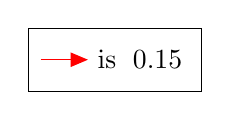
\begin{tikzpicture}
    \node at (0,0) (uses){is};
    \draw[->,red] ([xshift=-0.6cm]uses.west)  -- (uses.west);
    \node at ([xshift=0.4cm]uses.east) {\NeuralNetwork{0.15}};
    \draw[thin] (-1,-0.4) rectangle (1.2,0.4);
  \end{tikzpicture}
}

\begin{frame}{}
%  \myPaper{\footnotesize Ellis, Wong, Nye, ..., Solar-Lezama, Tenenbaum. 2020.}
  \centering
  \only<1>{

    \vspace{3cm}

    

    \hspace*{1cm}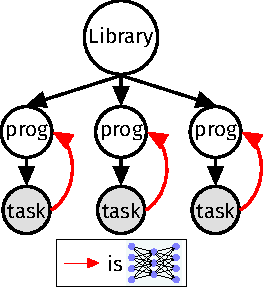
\includegraphics[width = 0.3\textwidth]{cycleGraphicalModel1}}
  \only<2>{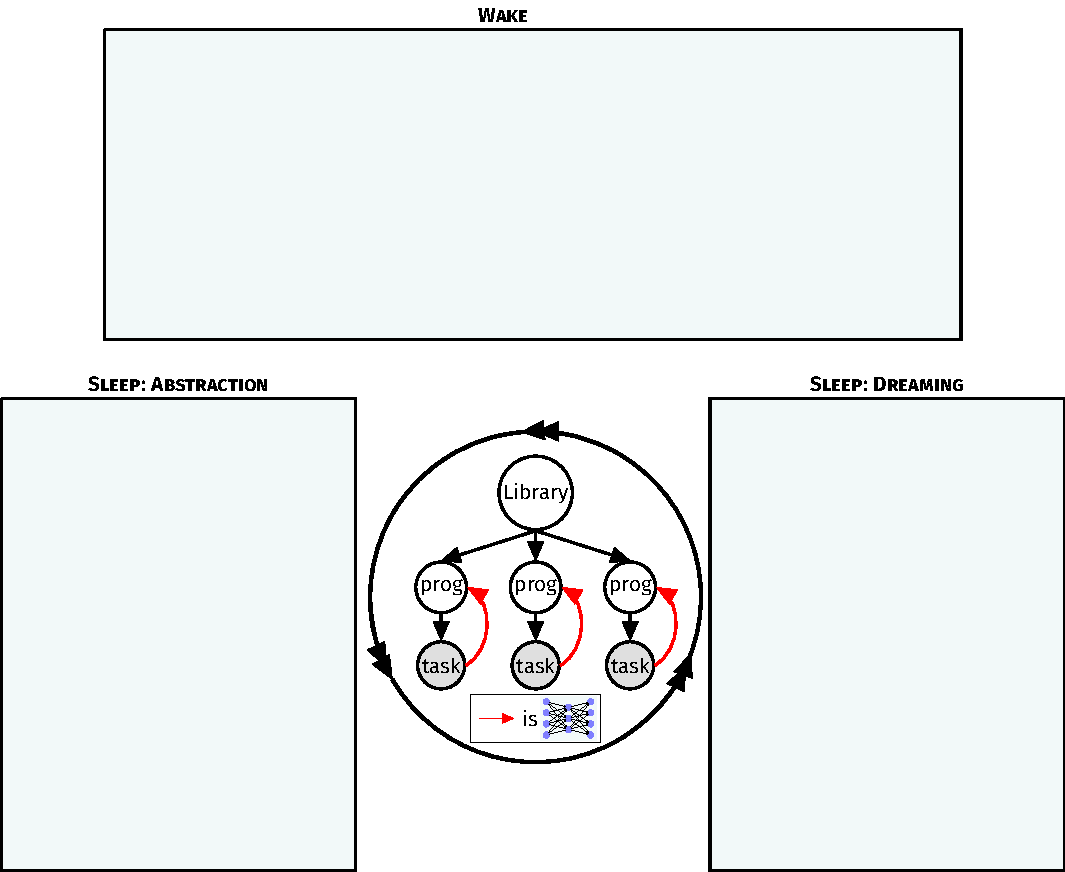
\includegraphics[width = \textwidth]{cycleGraphicalModel2}}
  \only<3>{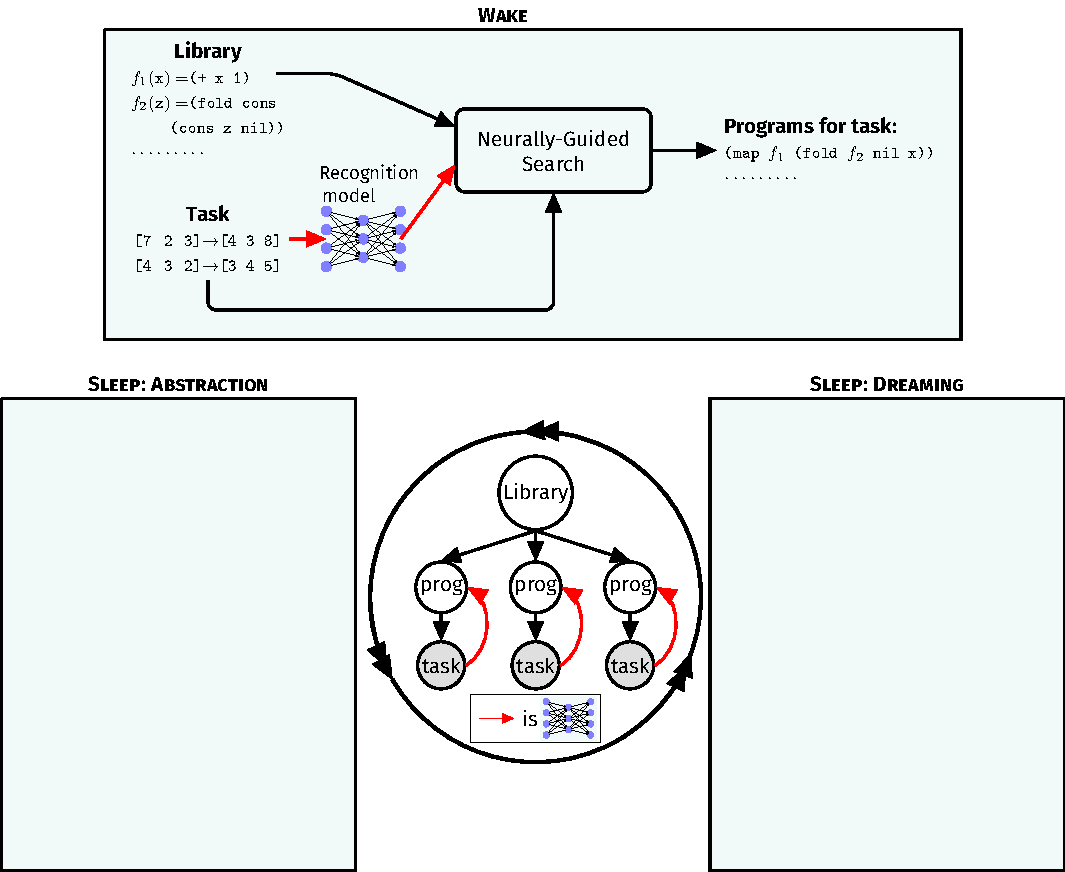
\includegraphics[width = \textwidth]{cycleGraphicalModel3}}
  \only<4>{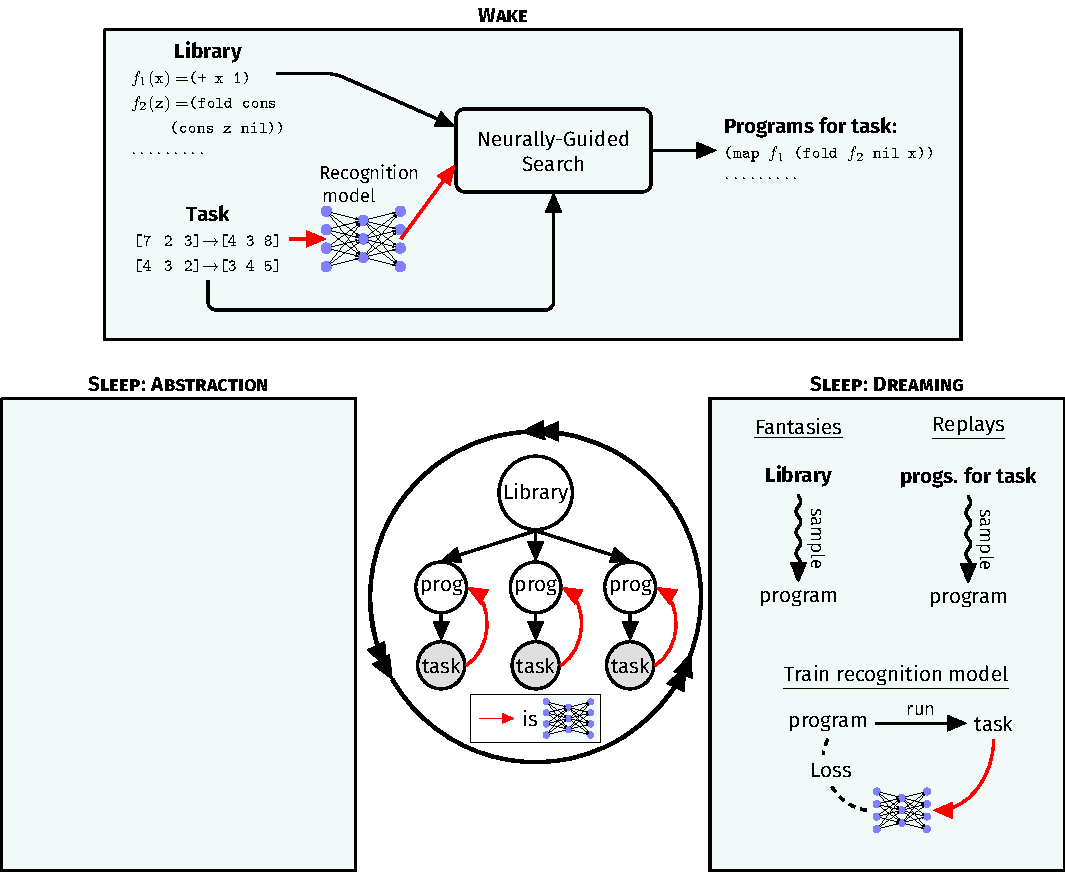
\includegraphics[width = \textwidth]{cycleGraphicalModel4}}
  \only<5>{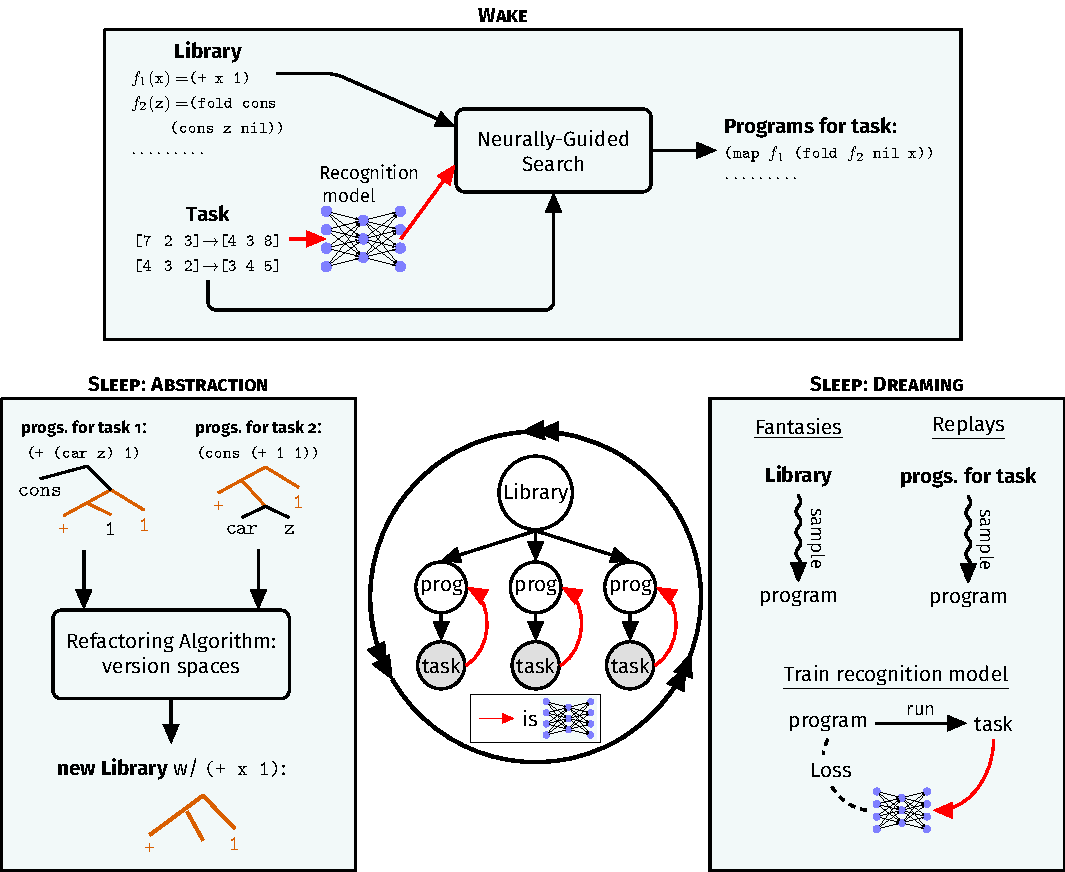
\includegraphics[width = \textwidth]{cycleGraphicalModel5}}
  \only<6>{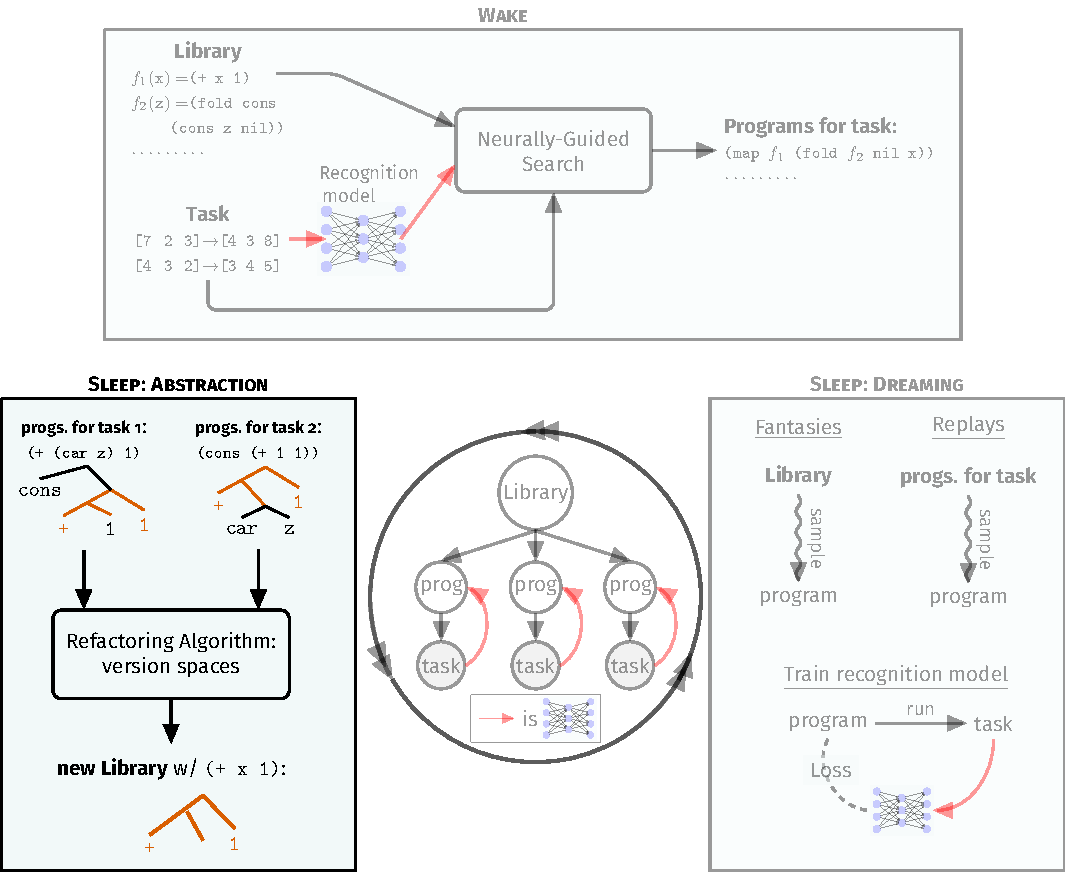
\includegraphics[width = \textwidth]{cycleGraphicalModelAbstraction}}
\end{frame}

\begin{frame}{Abstraction Sleep: Growing the library via refactoring}
  \centering
    \Wider[0em]{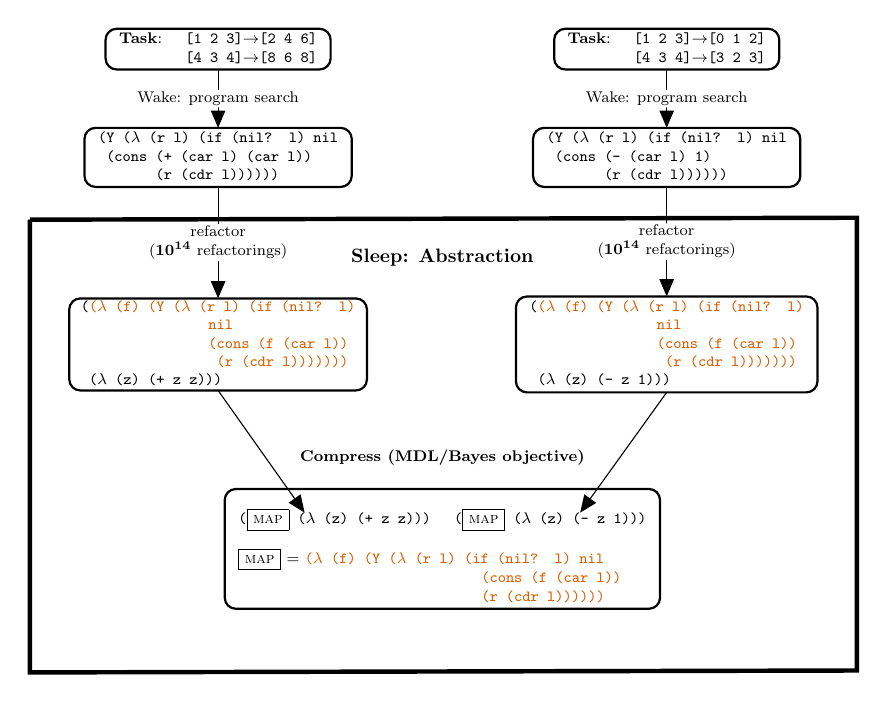
\begin{tikzpicture}[every node/.style={inner sep=1,outer sep=0,rounded corners,thick, scale=0.7}]
  \footnotesize
  \node(p1)[draw,rounded corners,thick] at (-1,0) {
    \begin{tabular}{l}
      \texttt{(Y ($\lambda$ (r l) (if (nil? l) nil}\\
      \texttt{ (cons (+ (car l) (car l))}\\
      \phantom{\texttt{(cons }}\texttt{ (r (cdr l))))))}
    \end{tabular}
  };
  
  \node(p2)[draw] at ([xshift=4cm]p1.east) {
    \begin{tabular}{l}
      \texttt{(Y ($\lambda$ (r l) (if (nil? l) nil}\\
      \texttt{ (cons (- (car l) 1)}\\
      \phantom{\texttt{(cons }}\texttt{ (r (cdr l))))))}
    \end{tabular}
    
  };

    \node(t1)[draw] at ([yshift=1cm]p1.north) {\begin{tabular}{ll}
      \textbf{Task}:&\texttt{[1 2 3]$\to$[2 4 6]}\\
      &\texttt{[4 3 4]$\to$[8 6 8]}
  \end{tabular}};
  \draw [->] (t1.south)  --(p1.north) node[fill=white,midway] {Wake: program search};
  \node(t2)[draw] at ([yshift=1cm]p2.north) {\begin{tabular}{ll}
      \textbf{Task}:&\texttt{[1 2 3]$\to$[0 1 2]}\\
      &\texttt{[4 3 4]$\to$[3 2 3]}
  \end{tabular}};
  \draw [->] (t2.south)  --(p2.north) node[fill=white,midway] {Wake: program search};

  
  \pause
  \node(r1)[draw,inner sep=0,outer sep=0] at ([yshift=-2cm]p1.south) {
    \begin{tabular}{l}
      \texttt{(}\orange{\texttt{($\lambda$ (f) (Y ($\lambda$ (r l) (if (nil? l)}}\\
      \phantom{(($\lambda$ (f) (Y ($\lambda$ (r l)}\orange{\texttt{nil}}\\
      \phantom{(($\lambda$ (f) (Y ($\lambda$ (r l)}\orange{\texttt{(cons (f (car l))}}\\
      \phantom{(($\lambda$ (f) (Y ($\lambda$ (r l)}\orange{\texttt{ (r (cdr l)))))))}}\\
      \texttt{ ($\lambda$ (z) (+ z z)))}
    \end{tabular}
  };

  \node(r2)[draw] at ([yshift=-2cm]p2.south) {
    \begin{tabular}{l}
      \texttt{(}\orange{\texttt{($\lambda$ (f) (Y ($\lambda$ (r l) (if (nil? l)}}\\
      \phantom{(($\lambda$ (f) (Y ($\lambda$ (r l)}\orange{\texttt{nil}}\\
      \phantom{(($\lambda$ (f) (Y ($\lambda$ (r l)}\orange{\texttt{(cons (f (car l))}}\\
      \phantom{(($\lambda$ (f) (Y ($\lambda$ (r l)}\orange{\texttt{ (r (cdr l)))))))}}\\
      \texttt{ ($\lambda$ (z) (- z 1)))}
    \end{tabular}

  };

  \draw [->] (p1.south)  --(r1.north) node[fill=white,midway,align=center] {refactor\\($\mathbf{10^{14}}$ refactorings)};
  \draw [->] (p2.south)  --(r2.north) node[fill=white,midway,align=center] {refactor\\($\mathbf{10^{14}}$ refactorings)};



    \node(dummy) at ($(0,1) + (r1.north)!0.5!(r2.north)$) {};
    \node(dummy1) at (r1.west) {\phantom{t}};


    \draw[ultra thick] ($(r1.north west) + (-0.5,1)$) -- ($(r2.north east) + (0.5,1)$)
    -- ($(r2.north east) + (0.5,1) + (0,-5.75)$)
    -- ($(r1.north west) + (-0.5,1) + (0,-5.75)$)
    -- ($(r1.north west) + (-0.5,1)$);
    %  \node(sleepBox)[ultra thick, rounded corners=0, inner sep=25,outer sep=20, draw, fit= (dummy) (r1) (r2) (m) (dummy1) ] {};
    \node at ($(0.0,0.5) + (r1.north)!0.5!(r2.north)$) {{\normalsize\textbf{Sleep: Abstraction}}};

    \pause
    
    \node[draw](m) at ($(0,-2) + (r1.south)!0.5!(r2.south)$) {
      \begin{tabular}{lr}
        &\\
        \code{(}\fbox{\textsc{map}}\code{ ($\lambda$ (z) (+ z z)))}&
        \code{(}\fbox{\textsc{map}}\code{ ($\lambda$ (z) (- z 1)))}\\&\\
        \multicolumn{2}{l}{\fbox{\textsc{map}} = \orange{\texttt{($\lambda$ (f) (Y ($\lambda$ (r l) (if (nil? l) nil}}}\\
        \multicolumn{2}{l}{\phantom{\texttt{\emph{map}} = \texttt{($\lambda$ (f) (Y ($\lambda$ (r l) (if }}\orange{\texttt{(cons (f (car l))}}}\\
        \multicolumn{2}{l}{\phantom{\texttt{\emph{map}} = \texttt{($\lambda$ (f) (Y ($\lambda$ (r l) (if }}\orange{\texttt{(r (cdr l))))))}}}
      \end{tabular}      
    };
    \draw [->](r1.south)--($(-1.75,-0.3) + (m.north)$);
    \draw [->](r2.south)--($(1.75,-0.3) + (m.north)$);
    \node[fill=white] at ([yshift=0.4cm]m.north) {\textbf{Compress (MDL/Bayes objective)}};

    \end{tikzpicture}}

    \only<4>{
      \messageOverlay{these $\mathbf{10^{14}}$ refactorings are manipulated using\\version spaces + equivalence graphs:\\exponentially more efficient refactoring data structure\\uses $\mathbf{10^{6}}$ nodes, calculated in $\leq $5min}
      }
\end{frame}

\begin{frame}{}
  \begin{center}
    \begin{tabular}{l}
      {\textcolor{black}{Program Induction and {\textcolor{gray}{learning to learn}}}}\\
      {\phantom{Program Induction and }\textcolor{gray}{learning a DSL}}\\
      {\phantom{Program Induction and }\textcolor{black}{learning to synthesize}}\\
      {\phantom{Program Induction and }{\textcolor{gray}{synergy between DSL+learned synthesizer}}}\\
    \end{tabular}
  \end{center}
\end{frame}

\begin{frame}
  \only<1>{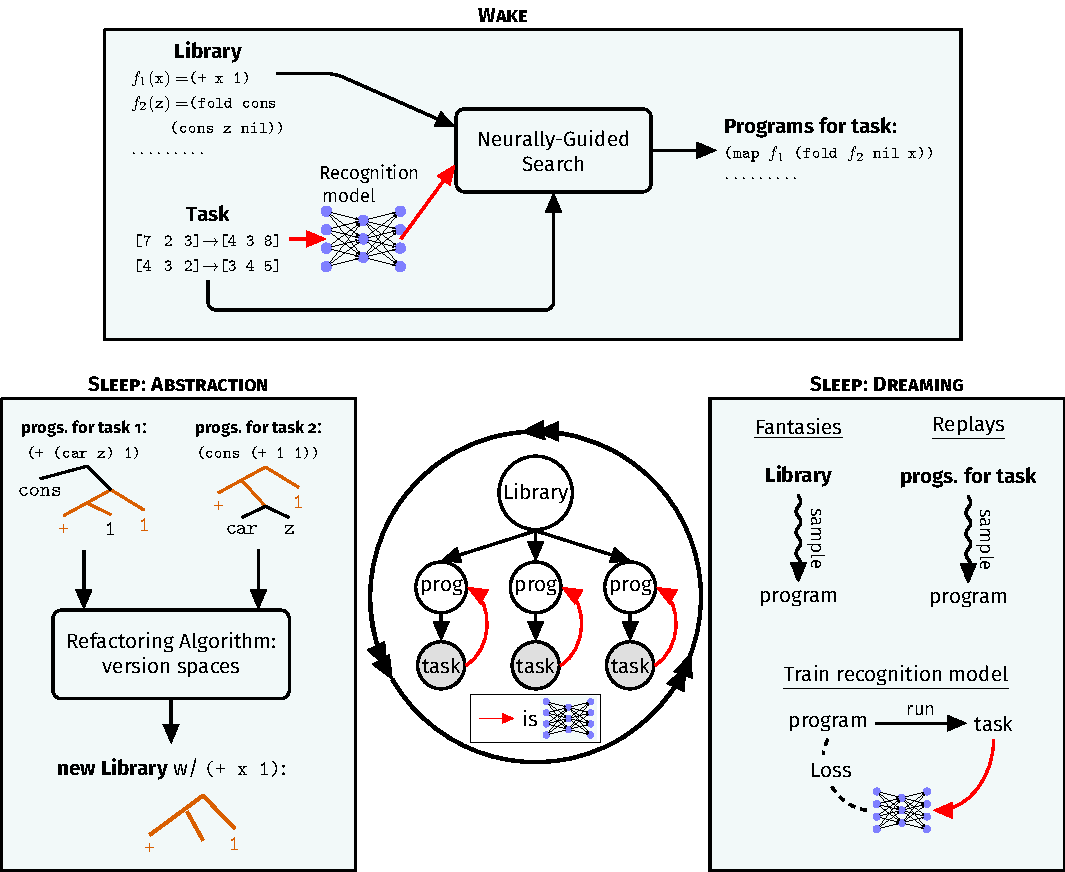
\includegraphics[width = \textwidth]{cycleGraphicalModel5}}
  \only<2>{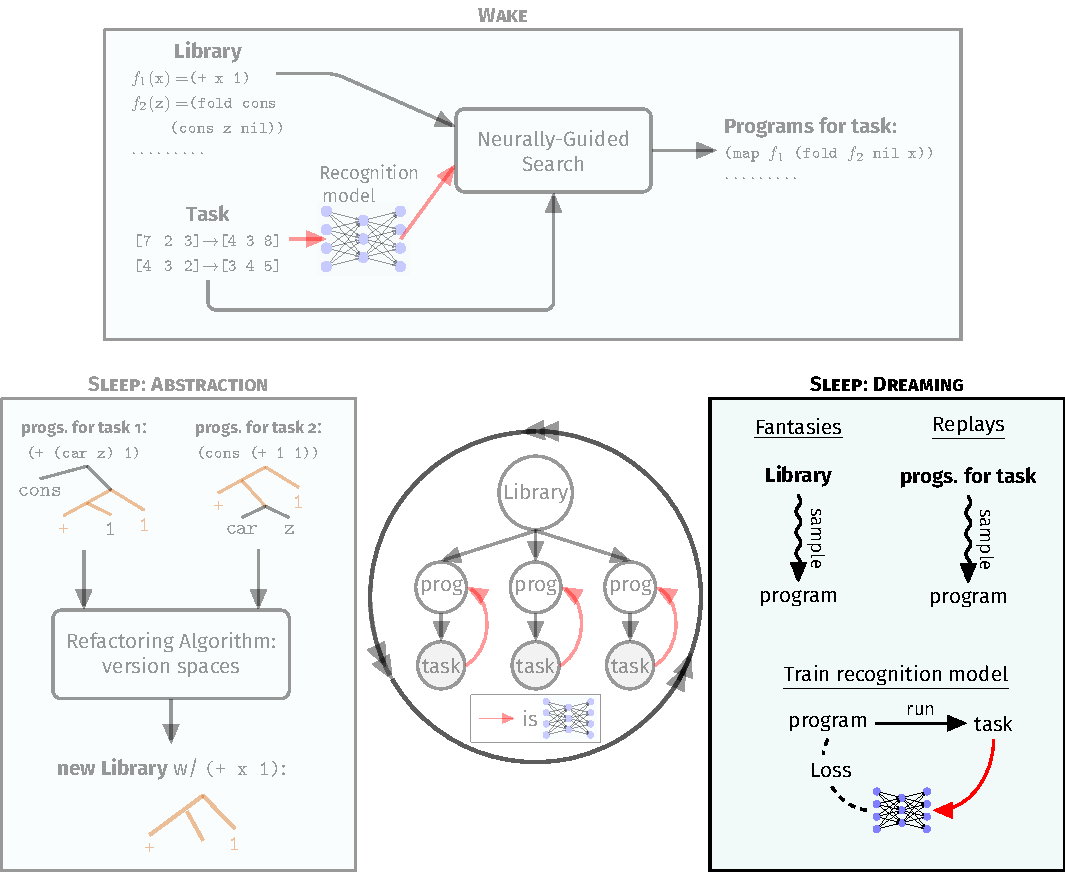
\includegraphics[width = \textwidth]{cycleGraphicalModelRecognition}}
\end{frame}

\begin{frame}[t]{Neural recognition model guides search}
  \vspace{1.2cm}
  \begin{tikzpicture}
    \node(t) at (0,0) {task};
    \node(n) at ([xshift=2cm]task.east) {
      \NeuralNetwork{0.17}};
    \node(p) at ([xshift=2cm]n.east) {program};
    \draw[thick,->] (t.east) -- ([xshift=-0.4cm]n.west);
    \draw[thick,->] ([xshift=0.4cm]n.east) -- (p.west);

    %% \node(n1) at ([yshift=-2cm]t.south) {\phantom{.}};
    %% \node[anchor=north west,align=left](c1) at ([xshift=0.5cm,yshift=0.3cm]n1.east) {\phantom{is a \textbf{``bigram'' model over syntax trees}}\\\phantom{test}\\\phantom{test}}\\\phantom{test}};
  \end{tikzpicture}

\end{frame}
\begin{frame}[t]{Neural recognition model guides search}
  \vspace{1cm}
  \begin{tikzpicture}
    \node(t) at (0,0) {task};
    \node(n) at ([xshift=2cm]task.east) {
      \NeuralNetwork{0.17}};
    \node(d) at ([xshift=2cm]n.east) {distribution};
    \draw[thick,->] (t.east) -- ([xshift=-0.4cm]n.west);
    \draw[thick,->] ([xshift=0.4cm]n.east) -- (d.west);
    \node(p) at ([xshift=2cm]d.east) {program};
    \draw[squiggle, thick,->] (d.east) -- node[sloped,above]{{{sample}}} (p.west);

    \pause

    \node(n1) at ([yshift=-2cm]t.south) {\NeuralNetwork{0.17}};
    \node[anchor=north west,align=left](c1) at ([xshift=0.5cm,yshift=0.3cm]n1.east) {is a...\\\phantom{is a...}recurrent network (Devlin et al 2017)\\
      \phantom{is a...}unigram model (Menon et al 2013; Balog et al 2016)};
  \end{tikzpicture}
\end{frame}
\begin{frame}[t]{Neural recognition model guides search}
  \vspace{1cm}
  \begin{tikzpicture}
    \node(t) at (0,0) {task};
    \node(n) at ([xshift=2cm]task.east) {
      \NeuralNetwork{0.17}};
    \node[align=left](d) at ([xshift=2cm]n.east) {distribution};
    \node[anchor=north] at (d.south) {{\tiny P(child$\vert$parent,arg)}};
    \draw[thick,->] (t.east) -- ([xshift=-0.4cm]n.west);
    \draw[thick,->] ([xshift=0.4cm]n.east) -- (d.west);
    \node(p) at ([xshift=2cm]d.east) {program};
    \draw[squiggle, thick,->] (d.east) -- node[sloped,above]{{{sample}}} (p.west);

    \only<1>{
      \node(n1) at ([yshift=-2cm]t.south) {\NeuralNetwork{0.17}};
      \node[anchor=north west,align=left](c1) at ([xshift=0.5cm,yshift=0.3cm]n1.east) {is a \textbf{``bigram'' model over syntax trees}};
    }

    \only<2->{
%      \node(l)[draw] at (2,-1) {\texttt{$\lambda$ (a)}};
      \node(k)[draw] at (1.7,-1.3) {\texttt{+}};
      \only<3->{
      \node(o)[draw] at ([xshift=-50,yshift=-50]k.south) {\texttt{9}};
      \draw[->] (k.south)--node[sloped, above]{\tiny P($\cdot \vert$ \texttt{+},\text{arg}=\text{left})}(o.north);
      }
      \only<4->{
        \node(m)[draw] at ([xshift=50,yshift=-50]k.south) {\texttt{*}};
        \draw[->] (k.south)--node[sloped, above]{\tiny P($\cdot \vert$ \texttt{+},\text{arg}=\text{right})}(m.north);
      }
      \only<5->{
        \node(x1)[draw] at ([xshift=50,yshift=-50]m.south) {\texttt{2}};
        \node(x2)[draw] at ([xshift=-50,yshift=-50]m.south) {\texttt{8}};

        %      \draw[->] (l.south)-- node[fill=white,align=center,midway,inner sep=0,outer sep=0]{$Q_{\text{start},\texttt{+},1}(x)$}(k.north);
        

        \draw[->] (m.south)--node[sloped, above]{\tiny P($\cdot \vert$ \texttt{*},\text{arg}=\text{left})}(x1.north);
        \draw[->] (m.south)--node[sloped, above]{\tiny P($\cdot \vert$ \texttt{*},\text{arg}=\text{right})}(x2.north);
      }

      \only<6>{
        \node[draw,rounded corners,ultra thick,align=left,anchor=north west] at (4.6,-0.7) {Why we do this:\\neural net runs once per task,\\\phantom{tt}so CPU bottlenecks instead of GPU};
      }
      \only<7>{
        \node[draw,rounded corners,ultra thick,align=left,anchor=north west] at (4.6,-0.7) {Advantages:\\neural net runs once per task,\\\phantom{tt}so CPU bottlenecks instead of GPU\\learns to break syntactic symmetries:\\\phantom{tt}P(1$\vert$\texttt{*},\text{arg}=\text{left})=0.0\\\phantom{tttt}``do not multiply by one''};
        }
    }
  \end{tikzpicture}
\end{frame}

\begin{frame}{}
  \begin{center}
    \begin{tabular}{l}
      {\textcolor{black}{Program Induction and {\textcolor{gray}{learning to learn}}}}\\
      {\phantom{Program Induction and }\textcolor{gray}{learning a DSL}}\\
      {\phantom{Program Induction and }\textcolor{gray}{learning to synthesize}}\\
      {\phantom{Program Induction and }{\textcolor{black}{synergy between DSL+learned synthesizer}}}\\
    \end{tabular}
  \end{center}
\end{frame}

\begin{frame}{DreamCoder Domains}
  \Wider[5em]{
    \only<1>{\includegraphics[width = \textwidth]{figures/manyDomainsLarger.png}}%{statement/taskbar2_expended.png}}
    \only<2>{\includegraphics[width = \textwidth]{figures/manyDomainsSelected.png}}%statement/taskbar2_selected.png}}
  }
  \myPaper{\small Ellis, Wong, Nye, ..., Solar-Lezama, Tenenbaum. arxiv 2020.}
\end{frame}

\begin{frame}{LOGO Turtle Graphics}
  30 out of 160 tasks
  \includegraphics[width = \textwidth]{dc/logoTasks30.png}
  \myPaper{\small Ellis, Wong, Nye, ..., Solar-Lezama, Tenenbaum. arxiv 2020.}
\end{frame}

\begin{frame}{LOGO Turtle Graphics}
  \begin{block}{DSL}
    \texttt{OP ::= FW x | RT x | UP | DOWN | SET state}
  \end{block}

  \begin{block}{Tasks}
    \texttt{task : image}
  \end{block}

  \vspace{0.2cm}

  \only<1>{
    \begin{columns}[T]
      \column{0.5 \textwidth}
        \begin{mycode}
          \texttt{FW 1}\\
          \vspace*{5\baselineskip}
        \end{mycode}
      \column{0.5 \textwidth}
        \includegraphics[width = 4cm]{../ecPaper/figures/teachLogo/line.eps}
    \end{columns}
  }
  \only<2>{
    \begin{columns}[T]
      \column{0.5 \textwidth}
        \begin{mycode}
          \texttt{FW 1}\\
          \texttt{RT} $\frac\pi2$\\
          \texttt{FW 1}\\
          \vspace*{3\baselineskip}
        \end{mycode}
      \column{0.5 \textwidth}
        \includegraphics[width = 4cm]{../ecPaper/figures/teachLogo/angle.eps}
    \end{columns}
  }
  \only<3>{
    \begin{columns}[T]
      \column{0.5 \textwidth}
        \begin{mycode}
          \texttt{FW 1}\\
          \texttt{RT} $\frac\pi2$\\
          \texttt{FW 1}\\
          \texttt{RT} $\frac\pi2$\\
          \texttt{FW 1}\\
          \vspace*{1\baselineskip}
        \end{mycode}
      \column{0.5 \textwidth}
        \includegraphics[width = 4cm]{../ecPaper/figures/teachLogo/angle2.eps}
    \end{columns}
  }
  \only<4>{
    \begin{columns}[T]
      \column{0.5 \textwidth}
        \begin{mycode}
          \texttt{for i in range(4)}\\
          \texttt{> FW 1}\\
          \texttt{> RT} $\frac\pi2$\\
          \vspace*{3\baselineskip}
        \end{mycode}
      \column{0.5 \textwidth}
        \includegraphics[width = 4cm]{../ecPaper/figures/teachLogo/square.eps}
    \end{columns}
  }
  \only<5>{
    \begin{columns}[T]
      \column{0.5 \textwidth}
        \begin{mycode}
          \texttt{for i in range(8)}\\
          \texttt{> FW 1} \\
          \texttt{> SET origin} \\
          \texttt{> RT} $\frac{2\pi}{8}$\\
          \vspace*{2\baselineskip}
        \end{mycode}
      \column{0.5 \textwidth}
        \includegraphics[width = 4cm]{../ecPaper/figures/teachLogo/star.eps}
    \end{columns}
  }
  \only<6>{
    \begin{columns}[T]
      \column{0.5 \textwidth}
        \begin{mycode}
          \texttt{for i in range(8)}\\
          \texttt{> PU} \\
          \texttt{> FW} $\frac{\text{\texttt{i}}}{2}$\\
          \texttt{> PD} \\
          \texttt{> FW} $\frac{\text{\texttt{i}}}{2}$\\
          \texttt{> RT} $\frac\pi2$\\
          \vspace*{0\baselineskip}
        \end{mycode}
      \column{0.5 \textwidth}
        \includegraphics[width = 4cm]{../ecPaper/figures/teachLogo/spiral.eps}
    \end{columns}
  }
  \only<7>{
    \begin{columns}[T]
      \column{0.5 \textwidth}
        \begin{mycode}
          \texttt{for i in range($\infty$)}\\
          \texttt{> FW $\varepsilon$}\\
          \texttt{> RT} $\varepsilon$\\
          \vspace*{3\baselineskip}
        \end{mycode}
      \column{0.5 \textwidth}
        \includegraphics[width = 4cm]{../ecPaper/figures/teachLogo/circle.eps}
    \end{columns}
  }
  \visible<7>{
    \vspace{0.2cm}
    \texttt{\alert{NUM} ::= 1 | $\pi$ | $\infty$ | $\varepsilon$ | + | - | * | / }
  }

    \end{frame}

\begin{frame}{LOGO Turtle Graphics -- learning an interpretable library}
  \Wider[5em]{
    \only<1>{\includegraphics[width = \textwidth]{dc/logo_kathy.png}}
    \only<2>{\includegraphics[width = \textwidth]{dc/logo_kathy_exploded1.png}}
    \only<3>{\includegraphics[width = \textwidth]{dc/logo_kathy_exploded2.png}}
    \only<4>{\includegraphics[width = \textwidth]{dc/logo_kathy_exploded3.png}}
    \only<5->{\includegraphics[width = \textwidth]{dc/logo_kathy.png}}
      
  }

  \only<6>{
  \messageOverlay{
    \begin{tabular}{rl}
    circle$(r)$
    &\raisebox{-.5\height}{\includegraphics[width = 0.3\textwidth]{dc/logo_primitives/circle_negative.png}}\\
    polygon$(n,\ell)$
    &\raisebox{-.5\height}{\includegraphics[width = 0.3\textwidth]{dc/logo_primitives/polygon_negative.png}}
  \end{tabular}
  }}
  \only<5>{
    \messageOverlay{\begin{tabular}{c}
    radial symmetry$(n,\text{body})$\\
    \includegraphics[width = 0.35\textwidth]{dc/rotationalmontage_negative.png}
  \end{tabular}}
  }
  \myPaper{\small Ellis, Wong, Nye, ..., Solar-Lezama, Tenenbaum. arxiv 2020.}
\end{frame}

\begin{frame}{What does DreamCoder dream of? (before learning)}
%  \emph{before} learning:
  \Wider[5em]{
    \begin{center}
      \includegraphics[height=\textheight]{dc/dreams/beforeLearning36}
    \end{center}
  }
%  \myPaper{Ellis, Wong, Nye, ..., Solar-Lezama, Tenenbaum. 2020.}  
  %  \includegraphics[height=3cm]{dc/dreams/cherry_picked/montageSeptember14}    
%    \end{tabular}}
    %% \only<2>{\begin{tabular}{lll}
    %%     before learning&&after learning\\
    %%     \includegraphics[width = 0.4\textwidth]{dc/dreams/appendixlogoinitial.png}&&
    %%     \includegraphics[width = 0.4\textwidth]{dc/dreams/appendixlogofinal.png}
    %%     \end{tabular}}
\end{frame}

\begin{frame}{What does DreamCoder dream of? (after learning)}
%  \emph{after} learning:
  \Wider[4em]{
    \begin{center}
      \includegraphics[height=\textheight]{figures/postDreams6}
    \end{center}
  }
%  \myPaper{Ellis, Wong, Nye, ..., Solar-Lezama, Tenenbaum. 2020.}  

%    \end{tabular}}
    %% \only<2>{\begin{tabular}{lll}
    %%     before learning&&after learning\\
    %%     \includegraphics[width = 0.4\textwidth]{dc/dreams/appendixlogoinitial.png}&&
    %%     \includegraphics[width = 0.4\textwidth]{dc/dreams/appendixlogofinal.png}
    %%     \end{tabular}}
\end{frame}

\begin{frame}{Planning to build towers}
  \myPaper{\small Ellis, Wong, Nye, ..., Solar-Lezama, Tenenbaum. arxiv 2020.}
  \Wider[5.5em]{
    \footnotesize
    \begin{tabular}{l}
      {example tasks (112 total)}\\
      \includegraphics[clip, trim = 0 0cm 0 2.9cm,width = 0.9\textwidth]{dc/tower_montage_21_negative.png}\\\\

    \end{tabular}
    \pause
    \begin{tabular}{l}
      {learned library routines ($\approx $ 20 total)}\\
      \begin{tabular}[t]{rlrl}
        arch$(h)$&%\begin{tabular}{l}
        \raisebox{-.1\height}{\includegraphics[width = 0.25\textwidth]{dc/tower/tower_dsl_towerArch.png}}&
        %\end{tabular}&
        pyramid$(h)$&
        \raisebox{-.1\height}{\includegraphics[width = 0.25\textwidth]{dc/tower/tower_dsl_pyramid.png}}
        \\
        wall$(w,h)$&
        \raisebox{-.3\height}{\includegraphics[width = 0.25\textwidth]{dc/tower/tower_dsl_bricks.png}}
        &%\\\\
        %% stairs$(h)$&\begin{tabular}{l}
        %%   \includegraphics[width = 0.25\textwidth]{dc/tower/tower_dsl_staircase.png}
        %% \end{tabular}\\\\
        \phantom{bbb}bridge$(w,h)$&
        \raisebox{-.3\height}{\includegraphics[width = 0.25\textwidth]{dc/tower/tower_dsl_bridge.png}}
        %\\\\\\
      \end{tabular}\\\\

  \end{tabular}}

  %% \pause

  %% \messageOverlay{
  %%   \begin{tabular}{ll}
  %%         \textbf{dreams before learning}&\textbf{dreams after learning}\\
  %%         \begin{tabular}{c}
  %%           \includegraphics[clip,trim = 0 4.5cm 0 0cm,width = 0.4\textwidth]{dc/tower/dreams/cherry_montage_initial_20.png}
  %%         \end{tabular}\phantom{testing}&
  %%         \begin{tabular}{c}
  %%           \includegraphics[clip,trim = 0 4.5cm 0 0cm,width = 0.4\textwidth]{dc/tower/dreams/cherry_montage_final.png}
  %%           \end{tabular}
  %%         \\\\
  %%     \end{tabular}
  %% }
\end{frame}

\begin{frame}{Dreams before learning}
  \includegraphics[clip,trim = 0 4.5cm 0 0cm,width = \textwidth]{dc/tower/dreams/cherry_montage_initial_20.png}
%  \myPaper{\small Ellis, Wong, Nye, ..., Solar-Lezama, Tenenbaum. 2020.}
\end{frame}

\begin{frame}{Dreams after learning}
  \includegraphics[clip,trim = 0 4.5cm 0 0cm,width = \textwidth]{dc/tower/dreams/cherry_montage_final.png}
%  \myPaper{\small Ellis, Wong, Nye, ..., Solar-Lezama, Tenenbaum. 2020.}
\end{frame}
\begin{frame}{Learning dynamics}
  \phantom{
  \small baselines: Exploration-Compression, EC [Dechter et al. 2013]
    \small \phantom{baselines: }neural program synthesis, RobustFill [Devlin et al. 2017]\phantom{otest}
    \small \phantom{baselines: }24 hours of brute-force enumeration
    }
  \begin{tabular}{lr}
    \begin{tabular}{l}
    \only<1>{\includegraphics[height = 2.29cm]{figures/revisedLearningCurves/tower_hits_ws_average_pretty_small_yl_stage1.png}}
    %    \only<2>{\includegraphics[height = 2.29cm]{figures/revisedLearningCurves/tower_hits_ws_average_pretty_small_yl_stage2.png}}
    \only<2>{\includegraphics[height = 2.29cm]{figures/tower_hits_ws_average_pretty_small_yl_ablationStage.png}}
%    \only<3>{\includegraphics[height = 2.29cm]{figures/revisedLearningCurves/tower_hits_ws_average_pretty_small_yl_stage3.png}}
    \only<3>{\includegraphics[height = 2.29cm]{figures/revisedLearningCurves/tower_hits_ws_average_pretty_small_yl.png}}
  \end{tabular}

    &

    \begin{tabular}{l}
      \only<2>{\includegraphics[width = 3cm]{figures/revisedLearningCurves/curveLegendTruncated.png}}
          \only<3>{\includegraphics[width = 3cm]{figures/revisedLearningCurves/curveLegend.png}}
  \end{tabular}
  \end{tabular}

  

  \visible<3>{
    \small baselines: Exploration-Compression, EC [Dechter et al. 2013]
    \small \phantom{baselines: }neural program synthesis, RobustFill [Devlin et al. 2017]\phantom{otest}
    \small \phantom{baselines: }24 hours of brute-force enumeration
    }


  %% }
  %% }
  \myPaper{\small Ellis, Wong, Nye, ..., Solar-Lezama, Tenenbaum. arxiv 2020.}
\end{frame}

\begin{frame}{Learning dynamics}
  \begin{tabular}{ll}
    \includegraphics[height = 2cm]{figures/revisedLearningCurves/text_hits_average_pretty_small_yl.png}
    %      \only<4->{\includegraphics[height = 2cm]{figures/revisedLearningCurves/text_hits_average_pretty_small_yl.png}}
    &
    \phantom{ttt}%
    \includegraphics[height = 2cm]{figures/revisedLearningCurves/logo_hits_average_pretty_small.png}\\
    \includegraphics[height = 2cm]{figures/revisedLearningCurves/tower_hits_average_pretty_small_yl.png}&
    \phantom{ttt}%
    \includegraphics[height = 2cm]{figures/revisedLearningCurves/rational_hits_average_pretty_small.png}\\
    \includegraphics[height = 2.29cm]{figures/revisedLearningCurves/list_hard_hits_ws_average_pretty_small_yl.png}
    &
    \phantom{tt.}%
    \includegraphics[height = 2.29cm]{figures/revisedLearningCurves/regex_marginal_test_unigram_gen_ws.png}
    %      \only<4->{\includegraphics[height = 2.29cm]{figures/revisedLearningCurves/regex_marginal_test_unigram_gen_ws.png}}%
    %    \includegraphics[height = 2.29cm]{figures/revisedLearningCurves/regex_marginal_test_unigram_gen_ws.png}%
    \phantom{tt}\includegraphics[width = 2.5cm]{figures/revisedLearningCurves/curveLegend.png}\hspace{-3cm}
  \end{tabular}

  \myPaper{\small Ellis, Wong, Nye, ..., Solar-Lezama, Tenenbaum. arxiv 2020.}
  %% }
  %% }

\end{frame}

\begin{frame}{Synergy between recognition model and library learning}
  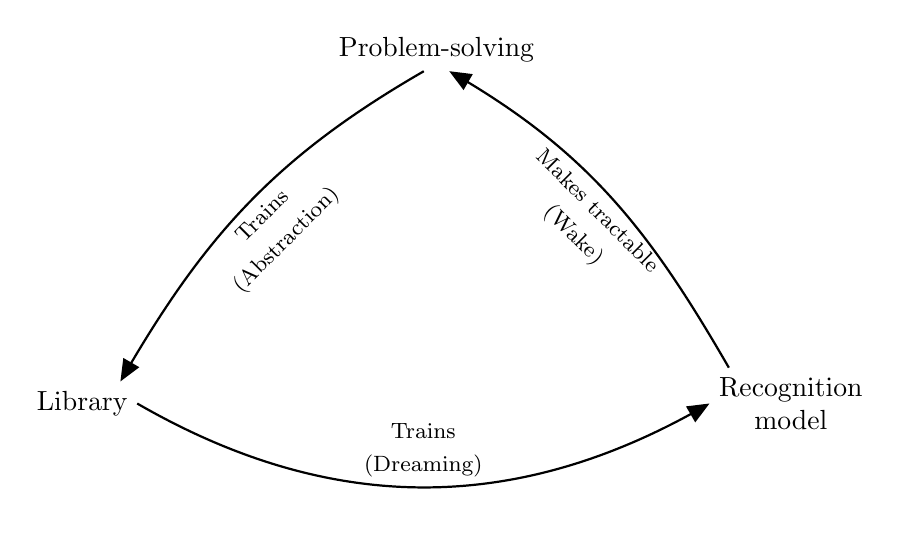
\begin{tikzpicture}[scale=1.5]
    {
    \begin{scope}[shift = {(1,-1)}]
    \node[align = center](synthesis) at (6,4) {Problem-solving};
    \node[align = center](Library) at (3,1) {Library};
    \node[align = center](recognitionModel) at (9,1) {Recognition \\model};

    \visible<2->{
      \draw [->,thick] (synthesis.-120) to[out = -150,in = 60] node[below,rotate = 45,align = center]{{\footnotesize Trains}\\{\footnotesize (Abstraction)}} (Library.30);
    }
    \visible<3->{
%      \draw [->,thick] (synthesis.-60) to[out = -30,in = 120] node[below,rotate=-45,align = center]{{\footnotesize Trains}\\{\footnotesize (Dreaming)}} (recognitionModel.150);
      \draw [->,thick] (Library.east) to[out = -30,in = 210] node[above, align = center]{{\footnotesize Trains}\\{\footnotesize (Dreaming)}} (recognitionModel.west);    
    }


    \visible<4->{
      \draw [->,thick] (recognitionModel.150) to[in = -30,out = 120] node[below,rotate=-45,align = center]{{\footnotesize Makes tractable}\\{\footnotesize (Wake)}} (synthesis.-60);
    }

    %% \visible<5->{
    %%   \draw [->,thick,dashed] (recognitionModel.north) to[out = 90,in = 0] node[fill=backgroundBeige,inner sep=1pt,align = center]{{\footnotesize Trains}\\{\footnotesize (Dreaming)}} (synthesis.east);
    %%   \draw [->,thick,dashed] (Library.north) to[out = 90,in = 180] node[fill=backgroundBeige,inner sep=0pt,align = center]{\footnotesize{Inductive bias}\\\footnotesize{(Wake)}
    %%   } (synthesis.west);
    %% }

  \end{scope}}
    \end{tikzpicture}
  \myPaper{\small Ellis, Wong, Nye, ..., Solar-Lezama, Tenenbaum. arxiv 2020.}
\end{frame}

\begin{frame}{Evidence for dreaming bootstrapping better libraries}
    \begin{tabular}{c}
      %        \multicolumn{1}{l}{\textbf{B}}\\
      \only<1>{\includegraphics[height = 0.3\textwidth]{figures/depthVersusAccuracy_revision_MEAN_blue.png}}
    \only<2->{\includegraphics[height = 0.3\textwidth]{figures/depthVersusAccuracy_revision_MEAN.png}}\\
{    \visible<2->{\includegraphics[height = 1cm]{figures/revisedLearningCurves/scatterLegend.png}}}
    \end{tabular}
    Darker: Early in learning

    Brighter: Later in learning
  \myPaper{\small Ellis, Wong, Nye, ..., Solar-Lezama, Tenenbaum. arxiv 2020.}
\end{frame}



%% \begin{frame}{Library structure: Probabilistic generative modeling of text}
%%   \Wider[5em]{\includegraphics[width = \textwidth]{deepArray2.pdf}}
%% \end{frame}

\begin{frame}{}

  {\huge
    From learning libraries,\phantom{tttesttesttest} \phantom{Fr} to learning languages}

  \vspace{2cm}

  \Wider[4em]{
    \visible<3>{\Large 1950's Lisp $\to $  }\visible<2->{\Large modern functional programming $\to $ physics}
  }
\end{frame}

\begin{frame}{}
  \begin{center}
    \includegraphics[width = 0.8\textwidth]{figures/PhysicsFormulas}
   \end{center}
\end{frame}

\begin{frame}{Growing languages for vector algebra and physics}
  \myPaper{\small Ellis, Wong, Nye, ..., Solar-Lezama, Tenenbaum. arxiv 2020.}
  \Wider[5em]{
    \only<1>{\includegraphics[width = \textwidth]{figures/physicsAnimation7}}
    \only<2>{\includegraphics[width = \textwidth]{figures/physicsAnimation6}}
    \only<3>{\includegraphics[width = \textwidth]{figures/physicsAnimation5}}
%    \only<4>{\includegraphics[width = \textwidth]{figures/physicsAnimation4}}
    \only<4>{\includegraphics[width = \textwidth]{figures/physicsAnimation3}}
    \only<5>{\includegraphics[width = \textwidth]{figures/physicsAnimation2}}
    \only<6>{\includegraphics[width = \textwidth]{figures/physicsAnimation1}}
  }
\end{frame}

\begin{frame}{Growing a language for recursive programming}
  \myPaper{\small Ellis, Wong, Nye, ..., Solar-Lezama, Tenenbaum. arxiv 2020.}\Wider[5em]{\only<1>{\includegraphics[width = \textwidth]{figures/mcCarthyAnimation5}}
    \only<2>{\includegraphics[width = \textwidth]{figures/mcCarthyAnimation4}}
    \only<3>{\includegraphics[width = \textwidth]{figures/mcCarthyAnimation3}}
    \only<4->{\includegraphics[width = \textwidth]{figures/mcCarthyAnimation2}}
%    \only<5>{\includegraphics[width = \textwidth]{figures/mcCarthyAnimation1}}
  }

  \vspace{-0.5cm}
  
  \visible<6>{\textbf{\Large 1 year of compute. 5 days on 64 CPUs.}}
  
  \visible<5->{
    \begin{tabular}{cc}
      \begin{tabular}{c}
        \includegraphics[width = 2cm]{figures/origamiCrane}
        \end{tabular}&\normalsize Origami Programming: Jeremy Gibbons, 2003
    \end{tabular}
  }
\end{frame}

\begin{frame}{Lessons}

  Symbols aren't necessarily interpretable. Flexibly grow the language based on experience to make it more powerful \emph{and} more human understandable

  \vspace{1cm}

  Learning-from-scratch is possible in principle. Don't do it. But program induction makes it convenient to build in what we know how to build in, and then learn and adapt on top of that

  \vspace{1cm}

  Some abstractions can be bootstrapped without language---but surely natural language supervision help...?
\end{frame}

\begin{comment}

  \begin{frame}{}
    \begin{center}
      \begin{tabular}{l}
        {\textcolor{black}{Program Induction and {\textcolor{gray}{learning to learn}}}}\\
        {\phantom{Program Induction and }\textcolor{gray}{learning a DSL}}\\
        {\phantom{Program Induction and }\textcolor{gray}{learning to synthesize}}\\
        {\phantom{Program Induction and }{\textcolor{black}{next steps}}}\\
      \end{tabular}
    \end{center}
  \end{frame}

  \begin{frame}{Some unresolved questions}

    Not everything is crisp and symbolic. How do we learn DSLs for neurosymbolic hybrid programs?\\(see Memoised Wake-Sleep, Hewitt et al 2020)

    \vspace{1cm}

    \pause

    Search is still hard\\(see ``REPL'': Ellis, Nye, Pu, Sosa et al 2019)

    \vspace{1cm}

    \pause

    Library$\not=$Language:\\
    How do we learn data structures, or discover new types, and thereby \emph{actually} learn DSLs?


  \end{frame}
\end{comment}



\newcommand{\closex}[2]{
  \renewcommand{\arraystretch}{#1}
  #2
  \renewcommand{\arraystretch}{1}
}
\newcommand{\closey}[2]{
  \setlength{\tabcolsep}{#1}
  #2
  \setlength{\tabcolsep}{6pt}
}

\newcommand{\person}[2]{\closex{0.2}{\begin{tabular}{c}
    {\footnotesize #1}\\
    \includegraphics[width = 1.7cm]{#2}
\end{tabular}}}

\begin{frame}{Collaborators}
\Wider[6em]{  \centering\begin{tabular}{ccc}
    \person{Josh\\{\footnotesize Tenenbaum}}{collaborators/Josh}&
    \person{Armando\\{\footnotesize Solar-Lezama}}{collaborators/Armando}&
    \person{Max Nye}{collaborators/MaxNye}\\\phantom{test}\\
    \person{Cathy Wong}{collaborators/cw}&
    \person{Mathias Sable-Meyer}{collaborators/French}&
    \person{Lucas Morales}{collaborators/Lucas}\\\phantom{test}\\
    \multicolumn{3}{c}{
    \begin{tabular}{c}
        \textbf{\Large thank}\\
        \textbf{\Large you}
    \end{tabular}}
    \end{tabular}}
  

\end{frame}


\begin{frame}[t]{3D program induction}
  \Wider[5em]{
    \begin{center}
      \includegraphics[width = \textwidth]{assets/we_are_cool_4.png}
    \end{center}
  }

    \vspace{1cm}
    
      Challenge: combinatorial search!\\
      Branching factor: $ > 1.3$ million per line of code, $\approx$ 20 lines of code\\
      search space size: $(1.3\text{ million})^{20}\approx 10^{122}$ programs
\myPaper{Ellis$^*$, Nye$^*$, Pu$^*$, Sosa$^*$, Tenenbaum, Solar-Lezama. NeurIPS 2019.\\$^*$equal contribution}

\end{frame}



\begin{frame}{}
  Solution: stochastic \textbf{tree search} + learn \textbf{policy} that writes code\\ + learn \textbf{value} function that assesses execution of program so far;\\
  analogous to \textbf{AlphaGo} [Silver et al. 2016]

  \Wider[5em]{
    \only<1>{\includegraphics[width = \textwidth]{figures/capitalism3.png}}
    \only<2>{\includegraphics[width = \textwidth]{figures/capitalism2.png}}
    \only<3>{\includegraphics[width = \textwidth]{figures/capitalism1.png}}
    \only<4>{\includegraphics[width = \textwidth]{figures/capitalism.png}}
  }
%  \myPaper{\tiny Ellis$^*$, Nye$^*$, Pu$^*$, Sosa$^*$, Tenenbaum, Solar-Lezama. NeurIPS 2019.\\$^*$equal contribution}
\end{frame}

\begin{frame}{3D program induction}
  \Wider[5em]{
    \begin{center}
      
      \setlength{\tabcolsep}{0pt}
      \renewcommand{\arraystretch}{0}  
      
      %    \includegraphics[width = \textwidth]{assets/pixel_montage} \\
      % \begin{tabular}{cc}
      %   \includegraphics[width = 0.3\textwidth]{assets/2d_synthetic_montage}&
      %   \includegraphics[width = 0.6\textwidth]{assets/tool_montage}
      % \end{tabular}\\\\    


        \begin{tabular}{ccccccc}
        \rotatebox[origin=l]{90}{Input}
        &    \rotatebox[origin=l]{90}{(voxels)}$\;$&
        \includegraphics[width = 2cm]{assets/3-D/demo3/spec}&
        %    \includegraphics[width = 2cm]{assets/3-D/demo6/0000png_v.png}&
        \includegraphics[width = 2cm]{assets/3-D/demo2/spec}&
        \includegraphics[width = 2cm]{assets/3-D/demo4/012_png_v.png}&
        \includegraphics[width = 2cm]{assets/3-D/demo5/CAD_example_input}&
        \includegraphics[width = 2cm]{assets/3-D/demo1/spec}
        \\
        \rotatebox[origin=l]{90}{Rendered}&
        \rotatebox[origin=l]{90}{program}$\;$&
        \includegraphics[width = 2cm]{assets/3-D/demo3/000_SMC_value_pickle_pretty.png}$\;$&
        %    \includegraphics[width = 2cm]{assets/3-D/demo6/2}$\;$&
        \includegraphics[width = 2cm]{assets/3-D/demo2/pretty}$\;$&
        \includegraphics[width = 2cm]{assets/3-D/demo4/012_SMC_value_pickle_pretty}$\;$&
        \includegraphics[width = 2cm]{assets/3-D/demo5/CAD_example_output}$\;$&
        \includegraphics[width = 2cm]{assets/3-D/demo1/pretty}
        \end{tabular}
      \setlength{\tabcolsep}{6pt}
      \renewcommand{\arraystretch}{1}
    \end{center}
  }

  \visible<2>{ same architecture learns to synthesize text editing programs (FlashFill, Gulwani 2012)}
  
  \myPaper{Ellis$^*$, Nye$^*$, Pu$^*$, Sosa$^*$, Tenenbaum, Solar-Lezama. NeurIPS 2019.\\$^*$equal contribution}

\end{frame}
\newcommand{\image}[2]{\includegraphics[#1]{../dreamcoder/figures/dpl/every/#2.pdf}}
\begin{frame}{Library structure: Text Editing}
  \Wider[5em]{
    DreamCoder learns libraries for FlashFill-style text editing  [Gulwani 2012]

    \vspace{0.5cm}

    \begin{tabular}{cc}
      \image{height=2.4cm}{text3}&
      \image{height=2.4cm}{text6}\\
      \image{height=2.4cm}{text5}&
      \image{height=2.4cm}{text4}
    \end{tabular}
  }
  \myPaper{\small Ellis, Wong, Nye, ..., Solar-Lezama, Tenenbaum. arxiv 2020.}
\end{frame}
\begin{frame}{Library structure: Generating Text}
  Libraries for probabilistic generative models over text:\\data from crawling web for CSV files

  
  \Wider[5em]{\begin{center}
    
    \begin{tabular}{cc}
      \image{height=3cm}{regex3}&
      \image{height=3.5cm}{regex1}\\
      \image{height=3.5cm}{regex2}&
      \image{height=3cm}{regex4}
    \end{tabular}
    \end{center}
  }
\end{frame}

\begin{frame}{150 random dreams before learning}
  \includegraphics[width = \textwidth]{../dreamcoder/figures/dreams/appendixlogoinitial.png}
\end{frame}
\begin{frame}{150 random dreams after learning}
  \includegraphics[width = \textwidth]{../dreamcoder/figures/dreams/appendixlogofinal.png}
\end{frame}
\end{document}
